\section{Приклади обчислень}
\begin{example}
Знайти ${\iint\limits_D y^3 x^2 d x d y}$, де через $D$ позначена область на площині обмежена лініями ${x = 0}$, ${y = x}$, ${x + y = 2}$.

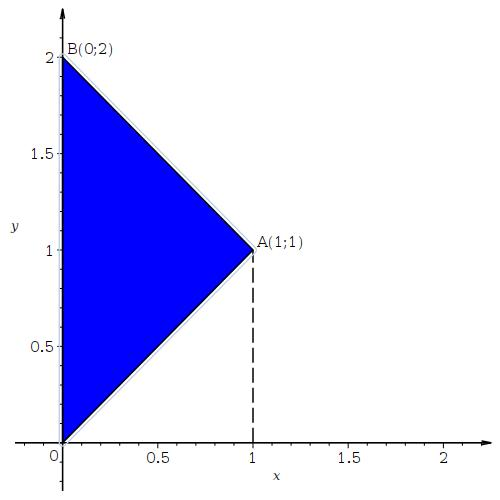
\includegraphics[width=0.5\paperwidth]{example.2.4}

Область $D$ є множиною на площині циліндричною в напрямку осі ${Oy}$, що визначається основою ${\left[0;1\right]}$. Для того, щоб знайти функції ${u_1, u_2\colon \left[0;1\right]\to \R}$, що визначають циліндричну множину $D$, потрібно записати рівняння ліній ${OA}$ і ${AB}$ --- ${y = x}$ і ${x + y =2 }$ відповідно, і виразити з них $y$ через $x$. Отримаємо
\[
\begin{array}{l}
u_1(x) = x,\\ u_2(x) = 2 - x.
\end{array}
\]
Згідно з теоремою про зведення кратного інтегралу до повторного маємо
\[
\iint\limits_D y^3 x^2 d x d y = \int\limits_0^1 \int\limits_{x}^{2 - x} y^3 x^2 d y d x.
\]
Спочатку знайдемо ${\int\limits_{x}^{2 - x} y^3 x^2 d y}$. З лiнiйностi iнтеграла Рiмана випливає, що
\[
\int\limits_{x}^{2 - x} y^3 x^2 d y = x^2 \int\limits_{x}^{2 - x} y^3  d y
\]
(пам’таємо, що iнтегрування вiдбувається по змiннiй $y$, тому змiнна $x$ при цьому є константою).

Тепер знайдемо первiсну:
\[
\int y^3  d y = \frac{y^4}{4} + C.
\]
Згідно з формулою Ньютона-–Лейбнiця:
\[
\int\limits_{x}^{2 - x} y^3 d y = \frac{y^4}{4}\biggr|_{y=x}^{2-x} = \frac{\left(2 - x\right)^4}{4} - \frac{x^4}{4}.
\]
Спростимо останній вираз:
\[
\begin{array}{c}
\dfrac{\left(2 - x\right)^4}{4} - \dfrac{x^4}{4} = \dfrac{2^4 - 4\cdot 2^3\cdot x^3 + 6\cdot 2^2\cdot x^2 - 4 \cdot 2\cdot x + x^4 - x^4}{4} =\\\\=\dfrac{16 - 32 x + 24 x^2 - 8 x^3}{4}  = 4 - 8 x + 6 x^2 -  2 x^3.
\end{array}
\]
Значить,
\[
\int\limits_{x}^{2 - x} y^3 x^2 d y = x^2 \int\limits_{x}^{2 - x} y^3  d y = x^2\left(4 - 8 x + 6 x^2 -  2 x^3\right) = 4 x^2 - 8 x^3 + 6 x^4 -  2 x^5,
\]
і
\[
\iint\limits_D y^3 x^2 d x d y = \int\limits_0^1 \left(4 x^2 - 8 x^3 + 6 x^4 -  2 x^5\right) d x.
\]
Знайдемо останній інтеграл.
\[
\begin{array}{c}
\int\limits_0^1 \left(4 x^2 - 8 x^3 + 6 x^4 -  2 x^5\right) d x =\\
\mbox{(лінійність)} \\
= 4 \int\limits_0^1 x^2  d x - 8 \int\limits_0^1x^3  d x + 6 \int\limits_0^1x^4  d x -  2 \int\limits_0^1x^5 d x  = \\
\mbox{(первісні і формула Ньютона--Лейбнiця)}\\
=4\cdot\dfrac{x^3}{3}\biggr|_0^1 - 8\cdot \dfrac{x^4}{4}\biggr|_0^1 + 6\cdot\dfrac{x^5}{5}\biggr|_0^1 - 2\cdot\dfrac{x^6}{6}\biggr|_0^1 =\\
\mbox{(рахуємо підстановки)}\\
= 4\cdot\dfrac{1^3}{3} - 8\cdot \dfrac{1^4}{4} + 6\cdot\dfrac{1^5}{5} - 2\cdot\dfrac{1^6}{6} - \left(4\cdot\dfrac{0^3}{3} - 8\cdot \dfrac{0^4}{4} + 6\cdot\dfrac{0^5}{5} - 2\cdot\dfrac{0^6}{6}\right) = \\\\
= \dfrac{4}{3} - 2 + \dfrac{6}{5} - \dfrac{1}{3} = \dfrac{1}{5}.
\end{array}
\]

У підсумку,
\[
\iint\limits_D y^3 x^2 d x d y = \dfrac{1}{5}.
\]
\end{example}

\begin{example}
Знайти ${\iint\limits_D \sin y d x d y}$, де через $D$ позначений трикутник на площині з вершинами ${A\left(1;\frac{\pi}{2}\right)}$, ${B\left(2;\frac{\pi}{2}\right)}$, ${C\left(3;\pi\right)}$.

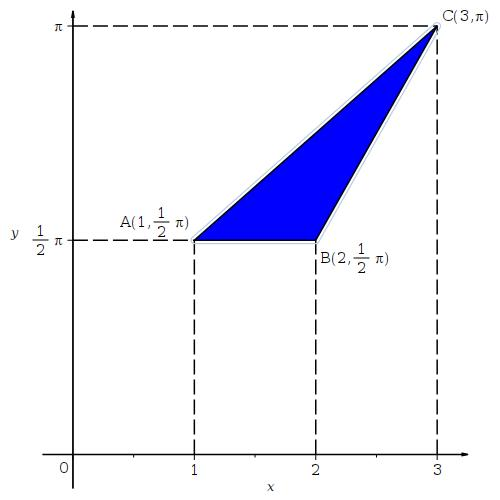
\includegraphics[width=0.5\paperwidth]{example.2.5}

Як і в попередньому прикладі, область $D$ є множиною на площині циліндричною в напрямку осі ${Oy}$. Основою в даному випадку буде відрізок ${\left[1;3\right]}$. Але функція ${u_1(x)}$ в цьому випадку записується двома різними формулами, що відповідають рівнянням прямих ${AB}$ і ${BC}$. Тому цей приклад має сенс ровз'язувати виходячи з того, що множина $D$ є також циліндричною в напрямку осі ${Ox}$. Основою тоді буде відрізок ${\left[\frac{\pi}{2};\pi\right]}$.
\begin{remark}
Якщо все ж таки розглядати множину $D$ як циліндричну в напрямку осі ${Oy}$, то отримаємо наступну рівність
\[
\iint\limits_D \sin y d x d y = \int\limits_{1}^{2}\left(\int\limits_{\frac{\pi}{2}}^{\frac{\pi}{2}+\frac{\pi  \left(x-1\right)}{4}}\sin y dy\right) dx+\int\limits_{2}^{3}\left(\int\limits_{\frac{\pi}{2}+\frac{\pi  \left(x-2\right)}{2}}^{\frac{\pi}{2}+\frac{\pi  \left(x-1\right)}{4}}\sin y dy\right) dx.
\]
Підрахуйте самостійно ці повторні інтеграли і переконайтесь, що відповідь буде така сама.
\end{remark}
Для того, щоб знайти функції ${u_1, u_2\colon \left[\frac{\pi}{2};\pi\right]\to \R}$, що визначають циліндричну множину $D$, потрібно записати рівняння ліній ${AC}$ і ${BC}$ --- ${\frac{\pi}{2}  x+2 y-\frac{\pi}{2} =0}$ і ${\frac{\pi}{2}  x-y-\frac{\pi}{2} =0}$ відповідно, але тепер виразити з них $x$ через $y$. Отримаємо
\[
\begin{array}{l}
u_1(y) = \frac{4 y - \pi}{\pi},\\ u_2(y) = \frac{\pi +2 y}{\pi}.
\end{array}
\]
Згідно з теоремою про зведення кратного інтегралу до повторного маємо
\[
\iint\limits_D \sin y d x d y = \int\limits_{\frac{\pi}{2}}^{\pi}\left(\int\limits_{\frac{4 y - \pi}{\pi}}^{\frac{\pi +2 y}{\pi}}\sin ydx\right) dy.
\]
Спочатку знайдемо ${\int\limits_{\frac{4 y - \pi}{\pi}}^{\frac{\pi +2 y}{\pi}}\sin ydx}$.

Знайдемо первiсну:
\[
\int \sin y dx = x\sin y + C
\]
(пам’таємо, що iнтегрування вiдбувається по змiннiй ${x}$, тому ${\sin y}$ при цьому є константою).

Згідно з формулою Ньютона-–Лейбнiця:
\[
\int\limits_{\frac{4 y - \pi}{\pi}}^{\frac{\pi +2 y}{\pi}}\sin ydx = x \sin y\biggr|_{x = \frac{4 y - \pi}{\pi}}^{\frac{\pi +2 y}{\pi}} = \frac{\pi +2 y}{\pi}\sin y - \frac{4 y - \pi}{\pi}\sin y = \frac{2\pi - 2 y}{\pi}\sin y.
\]

Значить,
\[
\iint\limits_D \sin y d x d y = \int\limits_{\frac{\pi}{2}}^{\pi}\frac{2\pi - 2 y}{\pi}\sin y dy.
\]
Знайдемо останній інтеграл.

Для цього нам потрібно буде використати формулу інтегрування частинами для визначених інтегралів:
\[
\int\limits_a^b u dv = u v \biggr|_a^b - \int\limits_a^b v du.
\]
\begin{align*}
&\int\limits_{\frac{\pi}{2}}^{\pi}\frac{2\pi - 2 y}{\pi}\sin y dy = &\\\\
&\left(\begin{array}{c}\mbox{ інтегрівання }\\ \mbox{ частинами }\end{array}\right)\left[\begin{array}{ll}u = \frac{2\pi - 2 y}{\pi} & \ \ \ dv = \sin y dy\\ du = \left(\frac{2\pi - 2 y}{\pi}\right)'dx = -\frac{2}{\pi}dx & \ \ \ v = \int \sin y dy = -\cos y\end{array}\right] = &\\\\
&= - \frac{2\pi - 2 y}{\pi} \cos y \biggr|_{\frac{\pi}{2}}^{\pi} - \int\limits_{\frac{\pi}{2}}^{\pi}\left(-\cos y\right)\left(-\frac{2}{\pi}\right)dx = & \\\\
&\mbox{(лінійність)} &\\\\
&= - \frac{2\pi - 2 y}{\pi} \cos y \biggr|_{\frac{\pi}{2}}^{\pi} - \frac{2}{\pi}\int\limits_{\frac{\pi}{2}}^{\pi}\cos ydx = &\\\\
&\mbox{(первісна і формула Ньютона--Лейбнiця)}&\\\\
&= - \frac{2\pi - 2 y}{\pi} \cos y \biggr|_{\frac{\pi}{2}}^{\pi} - \frac{2}{\pi}\sin y\biggr|_{\frac{\pi}{2}}^{\pi} = &\\\\
&\mbox{(рахуємо підстановки)}&\\\\
&= - \frac{2\pi - 2 \pi}{\pi} \cos \pi - \left(- \frac{2\pi - 2\cdot \frac{\pi}{2}}{\pi} \cos \frac{\pi}{2}\right) - \frac{2}{\pi}\sin \pi - \left(- \frac{2}{\pi}\sin\frac{\pi}{2}\right)=&\\\\
&\left(\cos\frac{\pi}{2}=0,\ \sin\pi = 0,\ \sin\frac{\pi}{2}=1\right)&\\\\
&=\frac{2}{\pi}.&
\end{align*}
У підсумку,
\[
\iint\limits_D \sin y d x d y = \frac{2}{\pi}.
\]
\end{example}
